\section{Experimento 4} 
Las principales aplicaciones de las celdas de carga son medir el peso de una masa (balanza)
y registrar la fuerza (contracción o expansión) entre dos puntos.
En este experimento se pretende observar la respuesta de la celda de carga, previo al acondicionamiento,
se realizarán mediciones a la salida diferencial para visualizar como responde a diferentes
cargas
\begin{figure}[H]
    \centering
    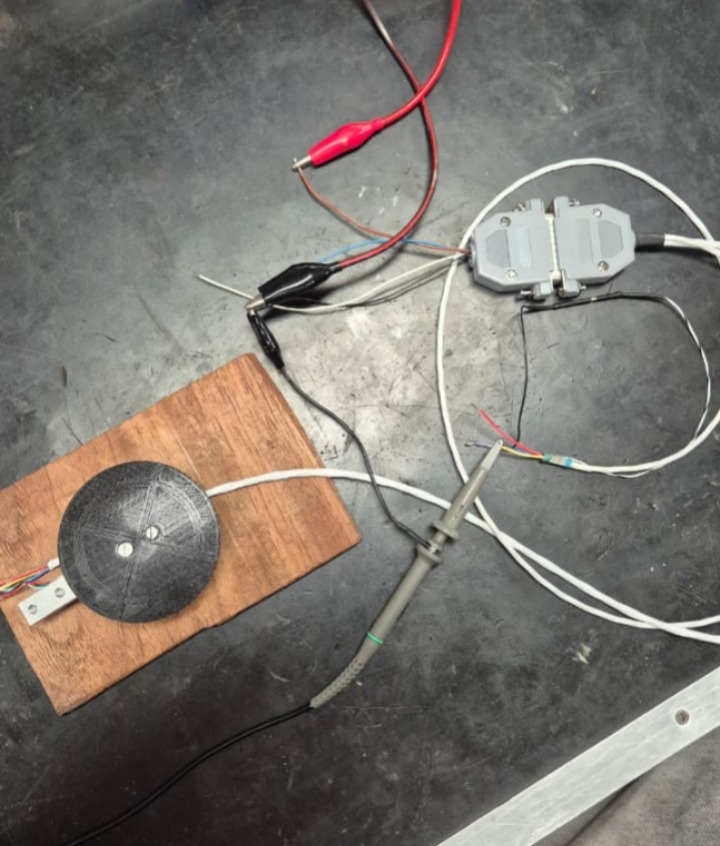
\includegraphics[width=0.5\textwidth]{images/exp4.jpeg}
    \caption{medición previa al acondicionamiento.}
    \label{fig:experimento4}
\end{figure}
Luego de todo el conexionado realizado, se procede a realizar las mediciones a la salida diferencial de la celda de carga, para diferentes cargas aplicadas, con el fin de observar la linealidad de la celda de carga y su respuesta a diferentes cargas.
Sin embargo previo al acondicionamiento, se observa que la celda de carga no responde de manera lineal a las cargas aplicadas, lo que indica que es necesario realizar un acondicionamiento previo para obtener mediciones precisas y confiables.

